\documentclass[11pt, a4paper]{article}
\usepackage[utf8]{inputenc}
\usepackage{graphicx}
\usepackage{setspace}
\usepackage{array}
\usepackage{fancyhdr}
\usepackage[none]{hyphenat}
\usepackage{rotating}
\usepackage{anyfontsize}
\usepackage{multirow}
\usepackage{listings}
\usepackage{xcolor}
\usepackage{float}
\usepackage[style=numeric-comp,hyperref=true,maxnames=6,sorting=none]{biblatex}
\addbibresource{references.bib}



\definecolor{codegreen}{rgb}{0,0.6,0}
\definecolor{codegray}{rgb}{0.5,0.5,0.5}
\definecolor{codepurple}{rgb}{0.58,0,0.82}
\definecolor{backcolour}{rgb}{0.95,0.95,0.92}

\lstdefinestyle{mystyle}{
    backgroundcolor=\color{backcolour},   
    commentstyle=\color{codegreen},
    keywordstyle=\color{magenta},
    numberstyle=\tiny\color{codegray},
    stringstyle=\color{codepurple},
    basicstyle=\ttfamily\footnotesize,
    breakatwhitespace=false,         
    breaklines=true,                 
    captionpos=b,                    
    keepspaces=true,                 
    numbers=left,                    
    numbersep=5pt,                  
    showspaces=false,                
    showstringspaces=false,
    showtabs=false,                  
    tabsize=2
}

\lstset{style=mystyle}

% For subfigures
\usepackage{caption}
\usepackage{subcaption}
% Get rid of the indent of the first line
\edef\restoreparindent{\parindent=\the\parindent\relax}
\usepackage{parskip}
% Fix text out of margin
\emergencystretch 3em
% Set date format
\usepackage[ddmmyyyy]{datetime}
% Set fonts
% \usepackage{fontspec}
% \setmainfont{Muli}[
%     Path = fonts/ ,
%     Extension = .ttf ,
%     UprightFont = *-Regular ,
%     ItalicFont = *-Italic ,
%     BoldFont = *-Bold ,
%     BoldItalicFont = *-BoldItalic
% ]
% \setsansfont{Muli-Black}[
%     Path = fonts/ ,
%     Extension = .ttf ,
%     ItalicFont = *Italic
% ]
% Set page margin
\usepackage{geometry}
\geometry{a4paper,
            % total={175mm,257mm}, %space for content
            headheight=80pt,
            headsep=2pt,
            % top=3cm,
            bottom=2.5cm,
            left=2cm,
            right=1.75cm}
% Set the name of the table of contents
\usepackage{url}                                                  % for correct typesettings of URLs
\usepackage{hyperref}                                             % for sophisticated linking of urls, dois, pictures, tables, etc.
\hypersetup{
    unicode=true,                                                 % non-Latin characters in Acrobat’s bookmarks
    pdftoolbar=true,                                              % show Acrobat’s toolbar?
    pdfmenubar=true,                                              % show Acrobat’s menu?
    pdffitwindow=false,                                           % window fit to page when opened
    pdfstartview={FitH},                                          % fits the width of the page to the window
    pdfauthor={C. Fortmann-Grote},                                           % author
    pdftitle={D5.4: VINYL software tested, documented, and released, including integration into interactive data analysis workflow with feedback loop},   % title
    pdfsubject={PaNOSC WP5 (ViNYL) Deliverable D5.4},                             % subject of the document
    pdfcreator={pdflatex},                                         % creator of the document
    pdfnewwindow=true,                                            % links in new PDF window
    colorlinks=true,                                              % false: boxed links; true: colored links
    linkcolor=black,                                                % color of internal links (change box color with linkbordercolor)
    citecolor=blue,                                                % color of links to bibliography
    filecolor=blue,                                               % color of file links
    urlcolor=blue                                                 % color of external links
}


\pagestyle{fancy}
\fancyhead{} % clear all header fields
\fancyfoot{} % clear all footer fields
\renewcommand{\headrulewidth}{0pt} % clear the header ruler line
\setlength{\footskip}{14pt}
\fancyfoot{} % clear all footer fields
\fancyfoot[R]{\hspace{1em}}
% \fancyfoot[c]{\begin{tabular}{c}
% 
\includegraphics[width=\textwidth, valign=b]{footer.pdf}& \\
% \end{tabular}}
\fancyfoot[L]{\hspace{1cm} 
\includegraphics[width=0.95\textwidth]{footer.pdf}}
% \cfoot{
\includegraphics[width=0.95\textwidth]{footer.pdf}}

% Set line spacing
\emergencystretch 3em
\setstretch{1.2}
% \setlength{\footskip}{10pt}

\begin{document}
% \thispagestyle{empty}
\chead{
\includegraphics[width=\textwidth]{header.pdf}}

{
	\centering
    \begin{onehalfspace}
    \sffamily
     \vspace*{5ex}
	{\fontsize{20}{24}\selectfont PaNOSC \par}
	{\fontsize{20}{24}\selectfont Photon and Neutron Open Science Cloud \par}
	{\fontsize{20}{24}\selectfont H2020-INFRAEOSC-04-2018 \par}
	{\fontsize{20}{24}\selectfont Grant Agreement Number: 823852 \par}
	\end{onehalfspace}

	\vspace*{7ex}
	
\includegraphics[width=\textwidth]{PaNOSClogo_web_RGB.pdf}\par
	\vfill
	{\large \textbf{\sffamily D5.4: VINYL software tested, documented, and released, including integration into interactive data analysis workflow with feedback loop}}\par
} % end of centering


\includegraphics[width=1.27in]{by.eps}\par
This work is licensed under a Creative Commons Attribution 4.0 International License\\
(\url{http://creativecommons.org/licenses/by/4.0/})\par

% \vspace*{0ex}
\newpage

% Set footer for the second page
% \setlength{\footnotesep}{50pt}
% \setlength{\footskip}{0pt}
\fancyfoot{} % clear all footer fields
\fancyfoot[R]{\thepage}
% \fancyfoot[c]{\begin{tabular}{c}
% 
\includegraphics[width=\textwidth, valign=b]{footer.pdf}& \\
% \end{tabular}}
\fancyfoot[L]{\hspace{1cm} 
\includegraphics[width=0.95\textwidth]{footer.pdf}}


{ %Front page
\restoreparindent
% \renewcommand{\arraystretch}{1.2} % change table row height

{\sffamily\huge Project Deliverable Information Sheet \par}

\begin{center}
\begin{tabular}{ | m{5.2cm}| m{10.7cm} | }
\hline
Project Reference No. & 823852 \\
\hline
Project acronym: & PaNOSC \\
\hline
Project full name: & Photon and Neutron Open Science Cloud \\
\hline
H2020 Call: & INFRAEOSC-04-2018 \\
\hline
Project Coordinator: & Andy Götz (andy.gotz@esrf.fr) \\
\hline
Coordinating Organization: & ESRF \\
\hline
Project Website: & www.panosc.eu \\
\hline
  Deliverable No: & D5.4: VINYL software tested, documented, and released, including integration into interactive data analysis workflow with feedback loop \\
\hline
Deliverable Type: & Report + Software \\
\hline
Dissemination Level: & Public \\
\hline
Contractual Delivery Date: & 30/11/2022 \\
\hline
Actual Delivery Date: & \today \\
\hline
EC project Officer: & Ren\'e Martins \\
\hline
\end{tabular}
\end{center}

{\large \textbf{Document Control Sheet} \par}
\begin{center}
\begin{tabular}{ | m{5.2cm}| @{}c@{} | }
\hline
\textbf{Document}
&
\begin{tabular}{| m{10.7cm} |}
  Title: D5.4:  VINYL software tested, documented, and released, including integration into interactive data analysis workflow with feedback loop \\\hline
Version: 1 \\\hline
Available at: \\\hline
Files: 1 \\\hline
\end{tabular}
\tabularnewline\hline
\textbf{Authorship}
&
\begin{tabular}{| m{10.7cm} |}
Written by: Carsten Fortmann-Grote \\\hline
Contributors:   Mads Bertelsen,
Stella d'Ambrumenil,
Juncheng E,
Aljo\v{s}a Hafner,
Gergely Norbert Nagy,
Shervin Nourbakhsh,
Mousumi Upadhyay Kahaly \\\hline
Reviewed by: Jordi Bodera Sempere\\\hline
Approved:  Andy Götz\\\hline
\end{tabular}
\tabularnewline\hline
\end{tabular}
\end{center}

{\large \textbf{List of participants} \par}
\begin{center}
    \begin{tabular}{|m{3.0cm}|m{9.5cm}|m{3cm}|}
        \hline
        \textbf{Participant No.} & \textbf{Participant organisation name} & \textbf{Country} \\
        \hline
        1 & European Synchrotron Radiation Facility (ESRF) & France \\
        \hline
        2 & Institut Laue-Langevin (ILL) & France \\
        \hline
        3 & European XFEL (XFEL.EU) & Germany \\
        \hline
        4 & The European Spallation Source (ESS) & Sweden \\
        \hline
        5 & Extreme Light Infrastructure Delivery Consortium (ELI-DC) & Belgium \\
        \hline
        6 & Central European Research Infrastructure Consortium (CERIC-ERIC) & Italy \\
        \hline
        7 & EGI Foundation (EGI.eu) & The Netherlands \\
        \hline
    \end{tabular}
\end{center}

}%End front page

% Table of contents
\newpage
\addtocontents{toc}{\protect\thispagestyle{fancy}}
\newpage
\tableofcontents
\newpage
% End Table of contents

\section{Abstract}
We report on the Deliverable D5.4 in work package 5 (Virtual Neutron and X--ray
Laboratory ---- ViNYL) in the European Union Horizon 2020 project \emph{Photon
  and Neutron Open Science Cloud ---- PaNOSC}. 
This report details the latest releases of  software developed under the umbrella of
ViNYL including test suites, documentation. In addition, we report on a use case
where ViNYL software is employed in an iterative data analysis workflow in serial
femtosecond crystallography. This is the final Deliverable.

\section{Introduction}

The main purposes of the PaNOSC work package 5 are to
harmonize the user interface for simulations of X-ray and neutron beamlines and
to enhance the interoperability of simulation codes using community
defined data formats and metadata standards. With the latest releases of
simulation code projects and simulation infrastructure libraries, these
ambitious
goals have now been accomplished. The present report aims at presenting a
comprehensive
overview on the various software solutions and gives references and pointers to
the respective resources for source code,
documentation and testing.

\section{libpyvinyl}
\label{sec:libpyvinyl}


\subsection{Scope and purpose}
\label{sec:lpv_scope}
libpyvinyl, the python APIs for Virtual Neutron and x-raY Laboratory, is a python package providing a way to harmonize the user interfaces of neutron and X-ray simulation codes by defining essential base and auxiliary classes for developers of a start-to-end simulation platform. 


\subsection{Current status of the project and contributions}
\label{sec:lpv_status}
libpyvinyl was developed mainly by the workpackage partners from
Eu.XFEL, ILL, and ESS, important feature requests and tests were contributed by
ESRF. To ensure that the library can fulfill its purpose as a harmonization
interface for various simulation backengines, it is vital that the library
continues to be developed in a decentralized manner at various places
representing a diversity of physics applications, simulation codes and use
cases. While the continuation of development of individual simulation codes and
APIs (such as McStasScript, SIMEX, or Oasys) is secured at the level of
individual RIs, this is, at the time of writing, much more uncertain in the case
of libpyvinyl. It would be desirable that the development teams of
individual simulation codes and frameworks can allocate sufficient resources to
the maintenance and development of libpyvinyl within their budgets.
Dedicated resources for the  library do currently not exist

\subsection{Structure of the library}
\label{sec:lpv_structure}
The structure of libpyvinyl is explained in detail in Deliverable D5.3
and in the documentation (see below in Sec~\ref{sec:lpv_repo}). We reiterate the
main concepts here:

\subsubsection{Main classes}
\label{sec:lpv_main_classes}

\begin{description}
\item[BaseCalculator] the interface to set parameters and perform calculation.
\item[BaseData]   the representation of the input/output data of a Calculator class.
\item[BaseFormat]   the interface to exchange data between the memory and the file on the disk in a specific format.
\end{description}

\subsubsection{Auxiliary classes}
\label{sec:lpv_aux}

\begin{description}
\item[Parameter] the Parameter class describes a single parameter with its limits (valid/invalid range) and unit (if applicable) defined.
\item[Calculator Parameters] a container for holding all the Parameter objects that pertain to a single Calculator.
\item[DataCollection] a thin layer interface between the Calculator and DataClass. It aggregates the input and output into a single variable, respectively.
\item[Instrument] a container for integrating different Calculator objects into a complete start-to-end simulation workflow.
\end{description}


\subsection{Repository}
\label{sec:lpv_repo}

The following table lists the relevant public resources for
libpyvinyl's source code, documentation site, testing status and use case.
\begin{table}[ht]
  \label{tab:lpv_repos}
  \centering
  \begin{center}
    \caption{Relevant libpyvinyl repositories.}
    \begin{tabular}{l p{10cm}l}
      \hline
      Source code repository & \url{https://github.com/PaNOSC-ViNYL/libpyvinyl} \\
      Release snapshots & \url{https://github.com/PaNOSC-ViNYL/libpyvinyl/releases}\\
      Documentation & \url{https://libpyvinyl.readthedocs.io}\\
      Test status  & \url{https://github.com/PaNOSC-ViNYL/libpyvinyl/actions/workflows/ci.yml}\\
      Usage illustration & \url{https://github.com/PaNOSC-ViNYL/libpyvinyl/tree/master/tests/integration/plusminus}\\
      \hline
    \end{tabular}
  \end{center}
\end{table}

The current release of libpyvinyl is
\href{https://github.com/PaNOSC-ViNYL/libpyvinyl/releases/tag/v1.1.2}{version 1.1.2}. Installation proceeds either from the cloned repository, from the
downloaded release tarball, or via the python package index as
\begin{lstlisting}[language=Python]
pip install libpyvinyl
\end{lstlisting}

\section{Instrument database}
\subsection{Scope and purpose}
Facility users have hardly access to complete and up--to--date instrument descriptions to run sample simulations and they are difficult to manipulate for a user not expert in the specific simulation software. 
The libpyvinyl API offers the high level interface to harmonize the interaction with an instrument described with different simulation softwares.
The instrument database has been designed to collect in a central place instrument descriptions created with softwares adopting the libpyvinyl API. Users are then able to access the instrument with few lines of code and run the simulation with a set of implemented samples (expandable). The instrument comes with the set of high level parameters defining the settings of the instrument that the user is supposed to be able to manipulate at the facility for the data acquisition, while all internal complexities are hidden.

\subsection{Current status of the project and contributions}
The structure of the database have been defined and a dedicated API is available to list its content and access the required instrument description.
Only few pilot instruments are described and are supposed to be used as examples for implementing new instruments.
A complete validation of the instruments has not been performed.

The instrument database and its API designs have been leaded by ILL and co-designed with ESS and EuXFEL.

%ESS have been involved in design of the instrument database and the structure of the API. 
It is envisioned several ESS instruments and sample environments will be submitted to the database soon, further testing and extending the system as needed. The instrument database will also address task 5.3 at a higher level of ambition than foreseen at the start of the project.

\subsection{Repository}
The database defined as a git repository hosted on the WP5 github organization as well as
he API to access the insturment database and make insturment descriptions available.

\href{https://github.com/PaNOSC-ViNYL/instrument_database}{https://github.com/PaNOSC-ViNYL/instrument\_database}


\href{https://github.com/PaNOSC-ViNYL/instrument_database_API}{https://github.com/PaNOSC-ViNYL/instrument\_database\_API}

\subsection{Structure}
\subsection{Maintainance and contribution policy}

\subsection{Installation and access}
The repository can be cloned in local using git commands:
\begin{lstlisting}[language=Python]
git clone  --recurse-submodules https://github.com/PaNOSC-ViNYL/instrument_database.git
\end{lstlisting}


\subsection{Documentation}
The documentation is self contained in the repository as Markdown file. 
The documentation targets both users of the instrument database and developers implementing instrument descriptions.

\subsection{Dissemination}
It is crucial to have a significant contribution from the research facilities by providing accurate and complete instrument descriptions and to maintain them.
A workshop dedicated to WP5 tools and prospects would be ideal to reach both expert and non-expert simulation users as well as developers.

\subsection{User base}
Currently limited but potentially every user submitting a proposal for beam time.



\section{McStasScript\label{sec:mcstasscript}}

For neutron scattering, the \href{https://www.mcstas.org}{McStas package} is the standard tool for instrument simulations, yet it has a
specialized user interface built on the C programming language. McStas has a
sister project called McXtrace that simulates X-ray instrumentation.
The McStasScript Python API that allows
nearly full access to McStas/\textit{McXtrace} features through an elegant Python
interface was mainly developed at the European Spallation Source (ESS). The main


\subsection{Scope and purpose of the package}
The McStasScript package aims to be an alternative user interface that covers the vast majority of McStas features. McStas itself is a Monte Carlo ray-tracing simulation code that covers neutron beamlines from source to detector, including sample scattering. Since the same software is used for the entire beamline, access to McStas from Python covers task 5.2 to 5.4, as it provides source simulation, beamline simulation and sample physics. Before McStasScript, McStas offered two ways of working with instrument simulations. Central to both are the instrument file that describes the instrument to be simulated in a C meta language. In this file the instrument is built from components and it is possible to have input parameters along with calculations. It is possible to run a simulation by using the command line tools to execute such a simulation by providing the instrument file, and then plot the resulting data using a different command line tool. McStas also provides a GUI with a text editor that provides some help features when inserting components, and then dialog boxes for running simulations and viewing the data. The data is always written to disk, usually as text files with metadata in a specialized format.

McStasScript thus provides a third way of writing McStas instruments, where everything can be done from the Python API. One defines an instrument object, adds components, parameters and calculations as necessary, and then runs the simulation from within the Python environment. The data is returned as objects with metadata and the numerical data is available as standard numpy arrays, making it easy to work with the generated data.

McStasScript was developed in parallel with the simulation base package
libpyvinyl in order to ensure a harmonization of the different simulation
package APIs. libpyvinyl provides base classes from which one can build
simulation packages, and these simulations packages will thus follow a similar
logic and share the most important method names. The libpyvinyl package is in
this way the answer to the harmonization part of task 5.1, and McStasScript is
built upon this base package.

\subsubsection{Repository}
The project is open source and available on the WP5 github repository. There are
two repositories, one for the main package and a separate one for example
notebooks, this makes it easier for users to get examples in a location more
easily accessible than the install location. Links to the repositories are shown
in table \ref{tab:links}. The McStasScript-notebook repository providez
simulation examples in the form of jupyter notebooks.

\begin{table}[h!!!]
\centering
\begin{tabular}{l|l}
Name & Link \\\hline
McStasScript & \href{https://github.com/PaNOSC-ViNYL/McStasScript}{https://github.com/PaNOSC-ViNYL/McStasScript} \\
McStasScript-notebooks &  \href{https://github.com/PaNOSC-ViNYL/McStasScript-notebooks}{https://github.com/PaNOSC-ViNYL/McStasScript-notebooks}
\end{tabular}
\caption{\label{tab:links} Links to McStasScript repositories.}
\end{table}

\subsubsection{Tests}
The package has good coverage with unit tests and these are used in continuous integration (CI). In addition, integration tests are available, as these do Monte Carlo simulations and require a local McStas installation, these are not included in CI.

\subsubsection{Installation}
It is possible to install the package through the Python package index pip as shown below. The package can also be installed from source by cloning the github repository. Regardless of the method, configuration is necessary to tell McStasScript where the local McStas/\textit{McXtrace} installation is located.

\begin{lstlisting}[language=Python]
pip install McStasScript
\end{lstlisting}

\subsubsection{Documentation}
The documentation is available at \href{https://mads-bertelsen.github.io}{https://mads-bertelsen.github.io}, where significant efforts have been made to provide comprehensive documentation. The documentation includes the purpose of the package, how to use it and tutorials on a large part of the McStas package as well as the McStas Union components. The release of the documentation along with online availability of the package was the ESS contribution to the completion of deliverable 5.2.

\subsubsection{Dissemination}
It is important to inform the community about the package in order to create a user community. Table \ref{tab:Dissemination} contains an overview of events where McStasScript was shown outside of PaNOSC events.

\begin{table}[h!!!]
\centering
\begin{tabular}{l|l}
Event & Format \\\hline
ECNS 2019 & Poster \\
ICANS 2019 & Poster and Presentation \\
SNS visit & Presentation for simulation group \\
HighNESS McStas course & Presentation \\
ISIS McStas course & Presentation \\
MLZ Garching group meeting & Presentation and online demo \\
PNPI group meeting & Presentation \\
ESS McStas days & Presentation and quiz exercises \\
ICNS 2022 & Poster and award speech for Instrumentation and Innovation prize \\
ESS-ILL User meeting 2022 & Poster \\
\end{tabular}
\caption{\label{tab:Dissemination} Overview of McStasScript dissemination activities.}
\end{table}

\subsubsection{User base}
It is difficult to judge the size of the current McStasScript user base as the download statistics include downloads of the package made through continuous integration, bots that mirror the package and so forth. There have been days with more than 300 downloads of the package, but it has not been possible to find a total number of downloads across all versions. Users provide issues to the github project, pull requests are being submitted and support requests are regularly received by the author over e-mail. It can be concluded that the package is reaching some level of adoption within the McStas/\textit{McXtrace} community. Known users are located at ILL, SNS, KU, DTU, MLZ, TUDelft and have even been used to design X-ray optics for space based telescope.

\subsection{McStasScript features}
This section aims to provide an overview of the feature set of McStasScript.

\subsubsection{Write instrument}
An instrument is made by creating an instrument object, and this instrument object can then have components added. These are a sequence of smaller codes that describe the beamline, and are each represented by a file on the users disk. McStasScript parses these files to internalize information on their parameters and units. It is possible to add components to any point in the sequence of components, but it is most common to place new components at the end. The instrument object inherits from the libpyvinyl calculator class in order to adhere to the standardized user interface created by WP5.

\subsubsection{Parameters}
It is also possible to add parameters to an instrument, these can be changed easily between runs. When changing components, McStas requires the underlying C code to be recompiled, but this can be avoided when only changing parameters. McStasScript has yet to implement code that avoids compiling when unnecessary, this is still the users responsibility.

\subsubsection{Error checking}
When writing a McStas instrument there are many possible ways to make an error that would result in the generated C code to fail to compile. A number of these are recognized by McStasScript and reported immediately instead of only when the user attempts to run the simulation. The exceptions raised by McStasScript are more specific that the compiler errors generated by McStas. Not all errors are caught, but the compiler output can be seen from McStasScript.

\subsubsection{Help features}
McStasScript contains a number of help features ranging from simple text overviews of the parameters, variables and components to diagrams of components included in an instrument. The help features can be used to find the right component in the library and to understand the parameters of components even before they are included in the instrument. When components are included in the instrument, colored text is used to show different states of the component parameters, such as default, required and set by user. The generated instrument diagrams such as seen in figure \ref{fig:diagram} are great for getting a quick overview of an instrument and are only available in McStasScript.

\begin{figure}[h!!!]
\centering
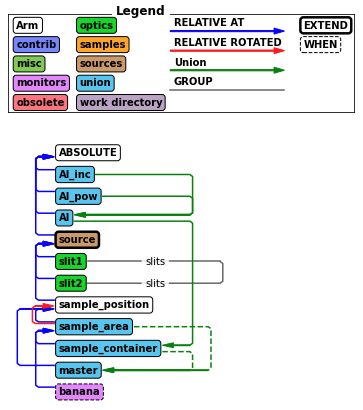
\includegraphics[width=0.5\textwidth]{figures/diagram_example.png}
\caption{\label{fig:diagram}Example of diagram from McStasScript. In widget mode one can hover the mouse over the left side of the boxes to see further info on each component.}
\end{figure}

\subsubsection{Run simulation}
The simulation can be executed from the Python environment, this is achieved with a system call using the subprocess module. The user can use the same controls available on the command line tools, such as setting the number of rays, location of data output, enabling gravity and selecting how many CPU cores will be used. The actual run method is called backengine to conform the libpyvinyl standard.

\subsubsection{Return of data}
Running a simulation returns data as a list of Python objects corresponding to each monitor in the instrument. These contain metadata such as the used parameters and information about the monitor as well as the actual data in nunmpy arrays. The objects also contain preferences on how this object should be plotted so the plotting tools in McStasScript can use appropriate settings when plotting the included data. 

\subsubsection{Widgets}
McStasScript also contains widgets specifically designed for use in Jupyter Notebooks. One widget can take a list of data objects and plot each of them with easy access to plot options and colorscales in the widget. The other widget takes an instrument object and is able to run the simulation with parameters set by the user, this widget shows the data from the simulation just as the plotting widget would. An example of the run widget can be seen in figure \ref{fig:widget}.

\begin{figure}
\centering
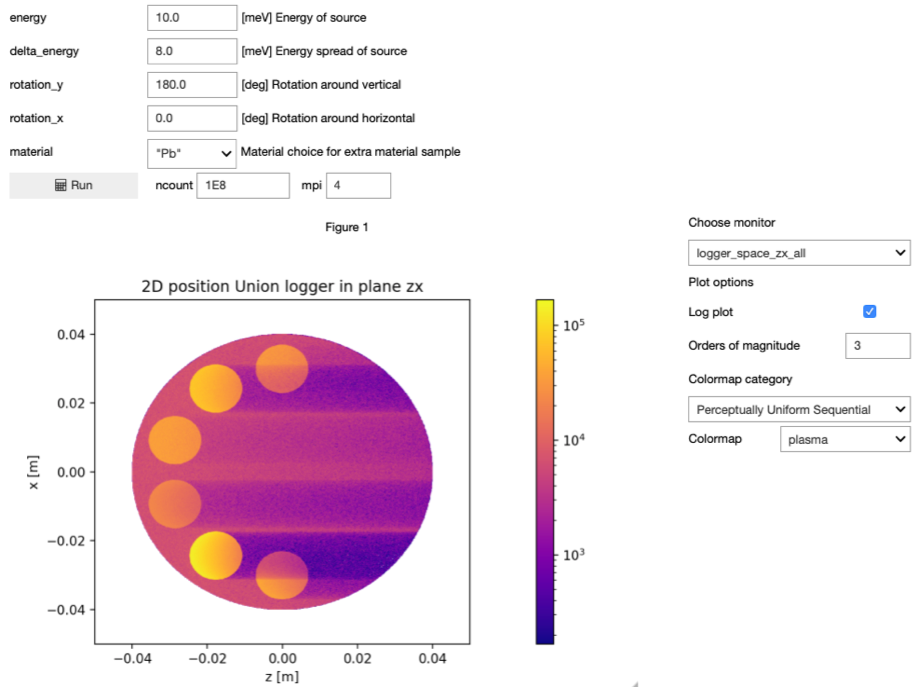
\includegraphics[width=0.9\textwidth]{figures/widget.png}
\caption{\label{fig:widget}Example of run widget from McStasScript. Here showing scattering in an imaging calibration sample with several embedded materials. Notice the streaks of lower intensity behind materials that scatter / absorb more than the others.}
\end{figure}

\clearpage
\section{openPMD\label{sec:openpmd}}
The openPMD \href{https://www.openpmd.org}{https://www.openpmd.org} format is to
be used for transferring descriptions of beams between different simulations
which was an objective of task 5.1 (see also the D5.1 report).
Core development of OpenPMD is not performed under the umbrella of WP5 but we
have contributed various domain specific extensions to the standard (molecular
dynamics, coherent wavefront propagation, x--ray and neutron raytracing). We mention
openpmd here only for the sake of completeness. Further details are given in the
D5.1 report.
\section{OASYS}

\subsection{Introduction}

OASYS (OrAnge SYnchrotron Suite) is an open source environment for modelling X-ray beamlines and experiments. It is based on Orange (\url{https://orangedatamining.com/}) framework which provides an easy-to-use graphical user interface (GUI). Various OASYS widgets (optical elements) are connected to each other, thus creating a workflow (beamline). This is particularly useful for X-ray optics simulations, as the wavefront propagation direction is well-defined and known in advance (from the source to the experimental station).

Several successful calculation packages exist and are actively maintained by the community. Among the most popular are \emph{SHADOW} for ray-tracing simulations and \emph{SRW} for wavefront propagation. During the PaNOSC project, we have addressed several different topics. This chapter provides an overview of all the development. All PaNOSC-specific widgets can be installed through OASYS1-PaNOSC (shown in Fig. \ref{fig:toolbox} package hosted on PyPI and available through the internal add-on manager. All contributions to the OASYS part described below come from CERIC-ERIC and ESRF.

\begin{figure}[htb]
    \centering
    \setkeys{Gin}{width=\linewidth}
    \begin{subfigure}{0.3\textwidth}
        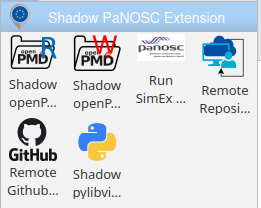
\includegraphics{figures/panosc_toolbox.png}
        \caption{}
        \label{fig:toolbox}
    \end{subfigure}
    \hfil
    \begin{subfigure}{0.5\textwidth}
        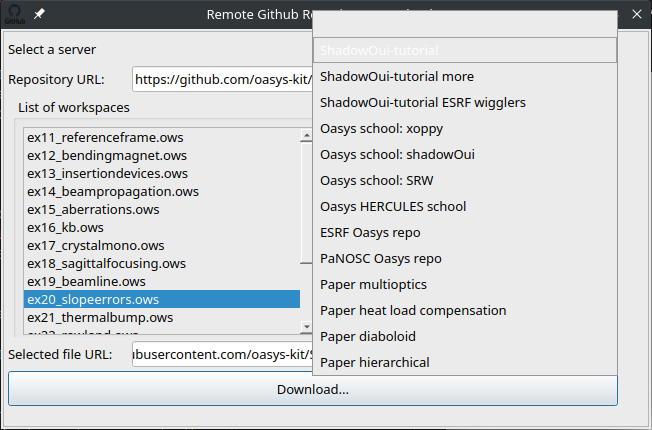
\includegraphics{figures/github_remote_access.png}
        \caption{}
        \label{fig:github_access}
    \end{subfigure}% trailing space between `subfigure` environments  had to be removed
    \caption{(a) PaNOSC widget toolbox. (b) Remote repository of OASYS workspaces (OWS) access through a widget in the GUI.}
\end{figure}

\begin{table}[ht]
  \label{tab:repos}
  \centering
  \begin{center}
    \caption{Relevant OASYS repositories. The current release of OASYS1-PaNOSC is \href{https://pypi.org/project/OASYS1-PaNOSC/0.3.2/}{v0.3.2} and of OASYS1-oasyswiser \href{https://pypi.org/project/OASYS1-oasyswiser/0.3.22/}{v0.3.22}.}
    \begin{tabular}{l p{10cm}l}
      \hline
      OASYS Panosc toolbox code & \url{https://github.com/PaNOSC-ViNYL/OASYS1-PaNOSC} \\
      Wiser (Library) repository & \url{https://github.com/oasys-elettra-kit/WISEr} \\
      OasysWiser (GUI) repository & \url{https://github.com/oasys-elettra-kit/OASYS1-Wiser} \\
      OASYS local Docker container & \url{https://gitlab.elettra.eu/panosc/ceric/oasys-local-docker} \\
      OASYS Jupyter Docker container & \url{https://gitlab.elettra.eu/panosc/jupyter-desktop-oasys} \\
      Dockerhub release & \url{https://hub.docker.com/r/ceric/panosc-oasys-local}\\
      E-learning Docker container & \url{https://github.com/pan-training/Docker/tree/main/wp8-summerschool} \\
      PaNOSC OWS database & \url{https://github.com/PaNOSC-ViNYL/Oasys-PaNOSC-Workspaces} \\
      \hline
    \end{tabular}
  \end{center}
\end{table}

\subsection{Wiser}

Wiser is a new package for wavefront propagation calculations based on Python implementation of WISE calculation code which stemmed from and is still maintained by Elettra Synchrotron. It is targeted at simulating the optical performance of X-ray mirrors. Propagation is done using Huygens-Fresnel integratal and allows for simultaneous 2-dimensional calculations of both figure errors (profiles) and roughness (statistical). Several optical elements have been implemented so far: plane mirror, elliptic mirror, spherical mirror, slit, detector, grating.

OASYS implementation consists of several abstraction layers of which the user interacts only with the top-most one - OASYS1-oasyswiser (available for installation on PyPI and through internal OASYS add-on manager). The back-end is a numerically optimized (able to use multi-core CPU processing) stand-alone Python library \emph{Wiser} which then interacts with \emph{WOFRY} package which strives to be a generic high-level abstraction of wavefront propagation workflows in OASYS. 

The development was done in three stages, it first focused on numerical optimization of Wiser. Since solving the Huygens-Fresnel integral is very expensive, this was a crucial step in usability and accessibility of the code. A few different optimization methods have been used. Using \emph{numba} Python library for just-in-time compiling of calculation kernel, a speed-up on the order of 10-100x has been reached. Afterwards, several new optical elements had to be implemented and a testing phase was conducted. When numerical consistency has been confirmed, work started on the GUI part. At present, all the elements beside the grating are available and ready-to-use as widgets in OASYS.

The package has been presented at the SPIE 2020 conference \cite{manfredda2020} and since then used in several applications (see Section \ref{subsec:panosc_use_cases}).

\subsection{COMSYL}

 COMSYL (COherent Modes for SYnchrotron Light) is a software package to perform numerically the coherent mode decomposition of undulator radiation in a storage ring \cite{Glass2017}. COMSYL requires the use of high-performance computer resources. COMSYL is used for beamline modelling at the ESRF-EBS. Several tasks that directly concern COMSYL have been carried out in the context of PaNOSC. COMSYL has evolved from the old OAR task manager to the new SLURM at the ESRF clusters. The OASYS add-on has also been updated. But, with no doubts, the most important and useful development concerns the development of a fast and lightweight tool for partially coherent beamline simulations \cite{SanchezdelRio2022} based on the same concepts of COMSYL, but fully implemented in python. This method has been thoroughly benchmarked against COMSYL and other tools used to simulate partially coherent x-rays \cite{SanchezdelRio2022}, and it is fully integrated in the OASYS package.

Not directly linked with COMSYL, but in the heart of OASYS, it is important to mention that the ray tracing engine SHADOW and the corresponding add-on ShadowOui have been upgraded to allow simulations for monochromators using crystals with high d-spacing \cite{Yu2022}, which is of particular interest for storages-rings producing soft X-rays.  

\subsection{Remote usage}

Being based on Orange which itself is using PyQT, OASYS is a standalone desktop application. By default it offers no remote access and/or collaborative development capabilites. A major portion of development has thus been focused on these features.

\subsubsection{Remote workspace access}

As part of PaNOSC deliverable D5.3, we have developed a widget for access to a remote repository of OWS workspaces (binary files in which OASYS projects are saved). The widget is able to read the file content of an arbitrary github repository where the files are be stored. The metadata description is read automatically from the workspace. It allows for access to several online repositories and opening of the workspace directly from within OASYS (Fig. \ref{fig:github_access}).

\subsubsection{Access to computing resources}
\label{sec:docker}

Running programs with rich GUIs remotely is non-trivial. One option is to use remote desktop solutions, but they are non-collaborative and require quite extensive user permissions. HPC servers normally also do not provide desktop environments. We have developed and experimented with several remote access options (see deliverable D5.2), but only the final one is presented and described here. A solution was developed through which arbitrary GUI software can be run as a Jupyter hub plugin as shown in Fig. \ref{fig:jupyter_select}. This links OASYS package with the rest of the WP5 simulation codes and can be installed into any existing Jupyter hub instance and allows OASYS to be run in a web browser (Fig. \ref{fig:oasys_run}), accessing any dedicated computing resources. This also avoids complex user permissions and relegates them to the Jupyter hub instance.

\begin{figure}[htb]
    \centering
    \setkeys{Gin}{width=\linewidth}
    \begin{subfigure}{0.3\textwidth}
        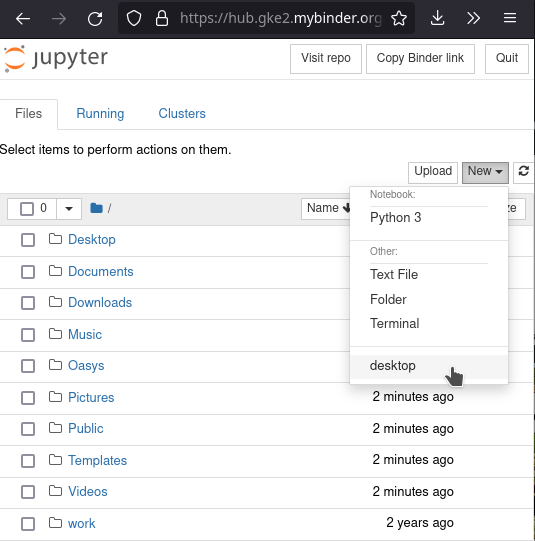
\includegraphics{figures/jupyter_select_desktop.png}
        \caption{}
        \label{fig:jupyter_select}
    \end{subfigure}
    \hfil
    \begin{subfigure}{0.5\textwidth}
        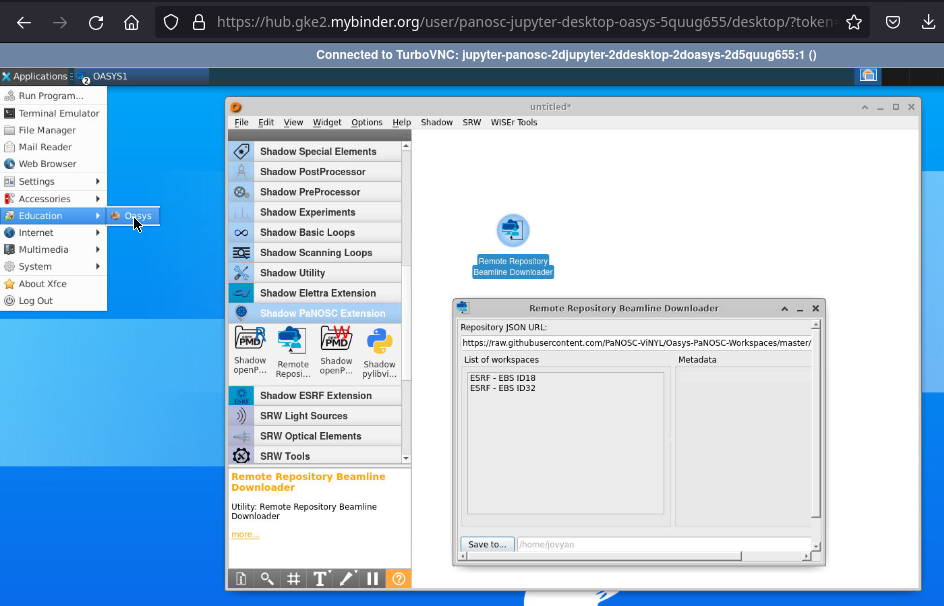
\includegraphics{figures/jupyter_oasys_run.png}
        \caption{}
        \label{fig:oasys_run}
    \end{subfigure}% trailing space between `subfigure` environments  had to be removed
    \caption{(a) Running the XFCE desktop environment from within Jupyter hub. (b) A new browser tab opens with XFCE desktop, providing a way to run OASYS inside the web browser while sharing the computing resources with the Jupyter hub instance.}
    \label{fig:oasysJupyter}
\end{figure}

\subsubsection{E-learning}

Building on the solution described in Sec. \ref{sec:docker}, a Docker container has been prepared for the purpose of E-learning. The said Docker container has been successfully used during the PaNOSC summer school organized by the training workpackage, WP8. It was further enriched with all necessary software for the course: Crispy, McStas and OASYS. Students could then seamlessly access all the required software without any installation on local machines and sharing the remote computing resources.

\subsection{openPMD}

As a part of task 5.1 and deliverable D5.1, we (CERIC-ERIC) have developed OASYS support for openPMD format and contributed to the standard for ray-tracing simulations. Two specific widgets, one for reading and one for writing openPMD files, are a part of the PaNOSC toolbox (Fig. \ref{fig:toolbox}).

\subsection{Beyond optics - Full beamline simulations}

Synergy between different simulation codes has been an important part of the developments in WP5. As OASYS simulates the X-ray spot parameters at various points along the beamline, the addition of beam-sample interaction through other codes was sought. Specifically, GAPD calculator found in Simex was used for demonstration purposes and is a part of deliverable D5.3. A prototype widget has been designed that can be seamlessly connected to the standard workflow. With this, one uses the result of X-ray propagation at the sample position and performs diffraction calculations on it. The architecture of the widget was further improved and it now allows for different calculators to be implemented in the future. A checking mechanism whether a given calculation code is properly installed on the system has also been implemented. The widget itself is shown in Fig. \ref{fig:widget1} and an example workflow in Fig. \ref{fig:workflow}.

\begin{figure}[htb]
    \centering
    \setkeys{Gin}{width=\linewidth}
    \begin{subfigure}{0.35\textwidth}
        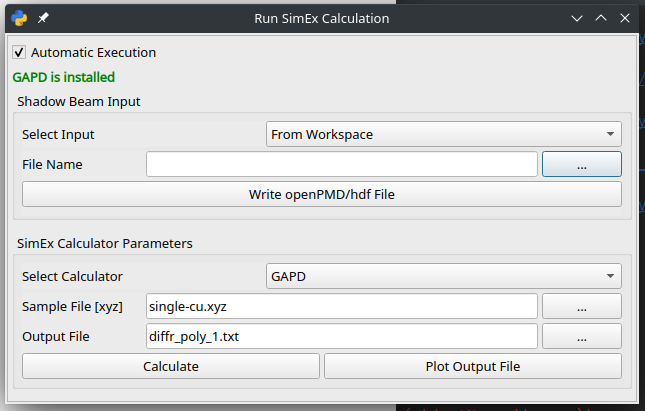
\includegraphics{figures/simexOasysWidget2.png}
        \caption{}
        \label{fig:widget1}
    \end{subfigure}
    \hfil
    \begin{subfigure}{0.55\textwidth}
        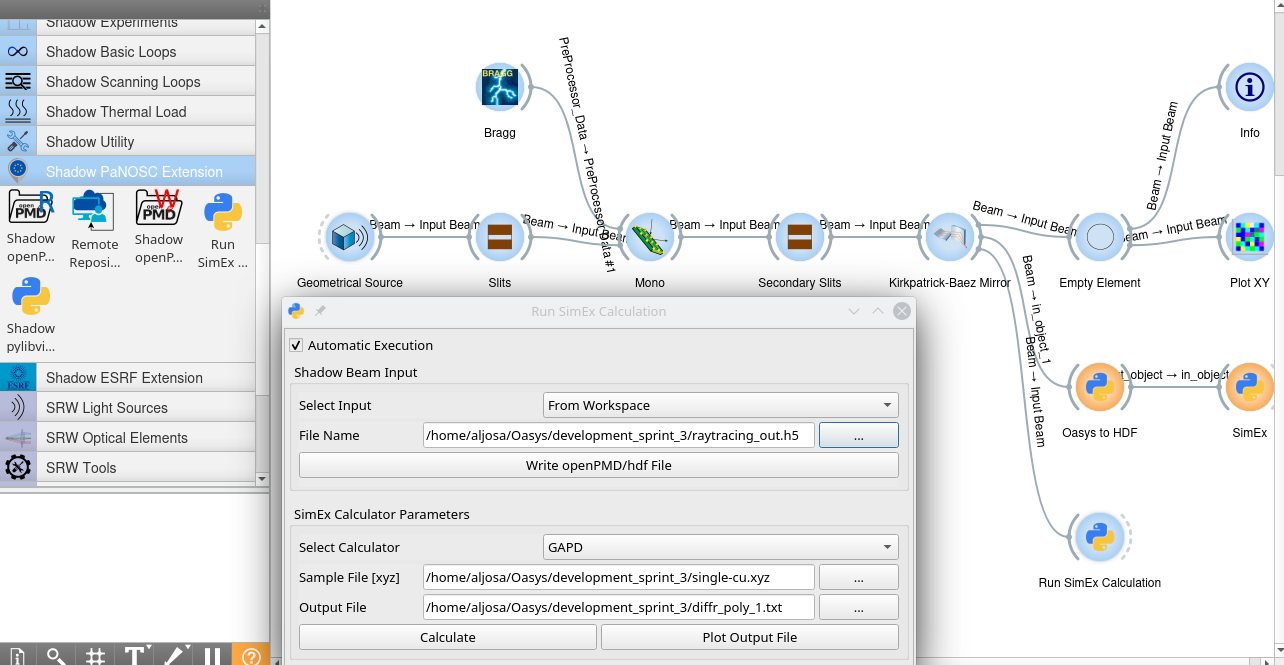
\includegraphics{figures/simexOasysWidget.png}
        \caption{}
        \label{fig:workflow}
    \end{subfigure}% trailing space between `subfigure` environments  had to be removed
    \caption{(a) Widget for running SimEx calculation directly from Oasys. (b) Example workflow where a beamline simulation result is used as an input to SimEx GAPD calculator.}
\end{figure}

\subsection{OASYS PaNOSC use cases}
\label{subsec:panosc_use_cases}
A list of use cases using OASYS, submitted to PaNOSC website is provided in Table \ref{tab:use_cases}. Our of 31 submitted use cases, 5 of them are either direct contributions to OASYS code or connected to infrastructural uses and setup of OASYS, i. e. remote access, e-learning, etc. This amounts to 16\% of all use cases, implying a significant impact in the community.

\begin{table}[h!!!]
\centering
\begin{tabular}{c l}
\# & Name \\\hline
8 & \href{https://www.panosc.eu/use-cases/use-case-8-remote-collaborative-access-to-beamline-optics-simulations/}{Remote, collaborative access to beamline optics simulations} \\
12 & \href{https://www.panosc.eu/use-cases/panosc-use-case-12-k-b-system-performance-analysis/}{K-B System performance analysis} \\
13 & \href{https://www.panosc.eu/use-cases/panosc-use-case-13-effects-on-the-spot-quality-of-mirror-error-profile-and-source-pointing-instability/}{Effects on the spot quality of the mirror error profile and source pointing instability} \\
16 & \href{https://www.panosc.eu/use-cases/panosc-use-case-16-coherent-mode-decomposition-of-synchrotron-emission-by-comsyl/}{Coherent mode decomposition of synchrotron emission by COMSYL} \\
31 & \href{https://www.panosc.eu/use-cases/use-case-31-seamless-connection-of-jupyter-notebooks-and-gui-applications-for-e-learning-purposes/}{Seamless connection of Jupyter notebooks and GUI applications for e-learning purposes}
\end{tabular}
\caption{\label{tab:use_cases} Links to PaNOSC use cases linked to OASYS. All use cases are published on \url{www.panosc.eu}.}
\end{table}


\section{SimEx-Lite\label{sec:simex-lite}}

SIMEX \cite{fortmann-grote2016} is a platform for simulation of experiments at advanced laser and X-ray light sources. SimEx-Lite is the core package of the SIMEX platform funded by the PaNOSC project to provide the calculator interfaces and data APIs for start-to-end simulation. By exposing all aspects of typical experiments at light source
infrastructures from the source to the detector, it allows to build a workflow to simulate behaviours of an X-ray instrument.  

\subsection{Repository}
SimEx-Lite is hosted at \url{https://github.com/PaNOSC-ViNYL/SimEx-Lite}, and its documentation can be found at \url{https://simex-lite.readthedocs.io/en/latest/}. The current release of SimEx-Lite is \href{https://pypi.org/project/SimEx-Lite/}{version-1.0.0}.

\subsection{Modules}
There are several calculator and data APIs already developed in SimEx-Lite. 

Calculators:
\begin{itemize}
    \item SourceCalculators
    \begin{itemize}
        \item GaussianSourceCalculator \cite{samoylova2016}
    \end{itemize}
    \item PropagationCalculators
    \begin{itemize}
        \item WPGPropagationCalculator \cite{samoylova2016}
    \end{itemize}
    \item PMICalculators (PhotonMattterInteractionCalculators)
    \begin{itemize}
        \item SimpleScatteringPMICalculator
    \end{itemize}
    \item DiffractionCalculators
    \begin{itemize}
        \item SingFELDiffractionCalculator \cite{pysingfel}
        \item CrystFELDiffractionCalculator \cite{white2012jac}
    \end{itemize}
    \item DetectorCalculators
    \begin{itemize}
        \item GaussianNoiseCalculator \cite{e2022}
    \end{itemize}
\end{itemize}

Data APIs:

\begin{itemize}
    \item WavefrontData
    \begin{itemize}
        \item WPGFormat
    \end{itemize}
    \item SampleData
    \begin{itemize}
        \item ASEFormat (For atomic structure formats supported by ASE)
    \end{itemize}
    \item PMIData (PhotonMatterInteractionData)
    \begin{itemize}
        \item XMDYNFormat
    \end{itemize}
    \item Diffractiondata
        \begin{itemize}
            \item SingFELFormat
            \item EMCFormat
        \end{itemize}
    \item DetectorData
        \begin{itemize}
            \item CXIFormat
        \end{itemize}
\end{itemize}

\subsection{Usage}
A calculator can be easily constructed within SimEx-Lite. Here, we take the\\
SingFELDiffractionCalculator as an example to explain its usage.

\begin{lstlisting}[language=Python]
from SimExLite.PMIData import PMIData, XMDYNFormat
from SimExLite.DiffractionCalculators import SingFELDiffractionCalculator

input_data = PMIData.from_file("./testFiles/PMI.h5", XMDYNFormat, "PMI_data")
diffraction = SingFELDiffractionCalculator(
        name="SingFELCalculator",
        input=input_data,)

print(diffraction.parameters)
\end{lstlisting}

With \verb|print(diffraction.parameters)| at the end, one can check the default values of the calculator's parameters. The output will look like this:

\begin{lstlisting}
 - Parameters object -
random_rotation                     True                 If it's False, the orientations...
calculate_Compton                   False                If calculate the compton...   
slice_interval                      100                  The slice interval of the pmi...  
slice_index_upper                   1                    The upper limit of the slice...
pmi_start_ID                        1                    The start ID of the pmi files   
pmi_stop_ID                         1                    The stop ID of the pmi files   
number_of_diffraction_patterns      10                   The number of diffraction...
pixel_size                          0.001      [meter]   The pixel size of the detector   
pixels_x                            10                   Number of pixels in x direction   
pixels_y                            5                    Number of pixels in y direction   
distance                            0.13       [meter]   Sample to detector distance   
mpi_command                         mpirun -n 2          The mpi command to run pysingfel
\end{lstlisting}

To run a simulation, as long as the corresponding backengine software is installed in the system, one can start the simulation with this function:
\begin{lstlisting}
output = diffraction.backengine()
\end{lstlisting}

The output is a data class mapping to the native output of the simulation software, with the \verb|output.get_data()| function, one can read the output data into memory as a python dictionary and conduct further analysis.

With different calculators representing different stages of an experiment, one can create an \verb|Instrument| instance to perform start-to-end simulation. An example is provided at
\url{https://github.com/PaNOSC-ViNYL/instrument_database/blob/spb/institutes/EuXFEL/instruments/SPB-SFX/HEAD/simex-lite/SPB-SFX.py}. One can load this defined instrument and run the defined simulation.

The packages integrated in the SIMEX platform have been applied in researches reported in several peer-reviewed publications\cite{fortmann-grote2017iucrj,e2021,e2022}.

% \begin{table}
% \centering
% % \begin{tabular}{| >{\centering\arraybackslash} m{8cm}| >{\centering\arraybackslash}m{6cm}|}
% \begin{tabular}{| >{\bfseries} m{7cm}|m{6cm}|}
% \hline
% SourceCalculators & GaussianSourceCalculator \\\hline
% PropagationCalculators & WPGPropagationCalculator \\\hline
% PMICalculators \newline (PhotonMattterInteractionCalculators) & SimpleScatteringPMICalculator \\\hline
% \multirow{2}{*}{DiffractionCalculators} & SingFELDiffractionCalculator \\\cline{2-2}
%  &  CrystFELDiffractionCalculator \\\hline
% DetectorCalculators & GaussianNoiseCalculator \\\hline

% \end{tabular}
% \caption{\label{tab:simexlite} Calculators developed in SimEx-Lite by Nov 17, 2022.}
% \end{table}


\section{Integrated simulation data workflows\label{sec:simdata}}
EXtra-xwiz is a command-line tool for automated processing of the calibrated serial crystalography data\cite{xwiz}. As described in the Task 5.5 of the proposal of Work Package 5, we have created a workflow to couple SimEx-Lite and EXtra-xwiz together to optimize instrument parameters for serial femtosecond crystallography (SFX) experiments by analyzing the simulation data from SimEx-Lite with EXtra-xwiz. 

As the schematic of the workflow shown in Fig.~\ref{fig:feedbackloop}, the simulation parameters and sample structure (can be any format compatible with the PDB format) are set for the CrystFEL calculator in SimEx-Lite. After running the simulation, the diffraction patterns output in CXI format is analysed by EXtra-xwiz. By making use of the metrics obtained with EXtra-xwiz, we can optimize the parameters to maximize the metric of interest in a certain condition. The optimized parameters can be a useful reference to achieve better experiment quality.

\begin{figure}[h!!!]
    \centering
    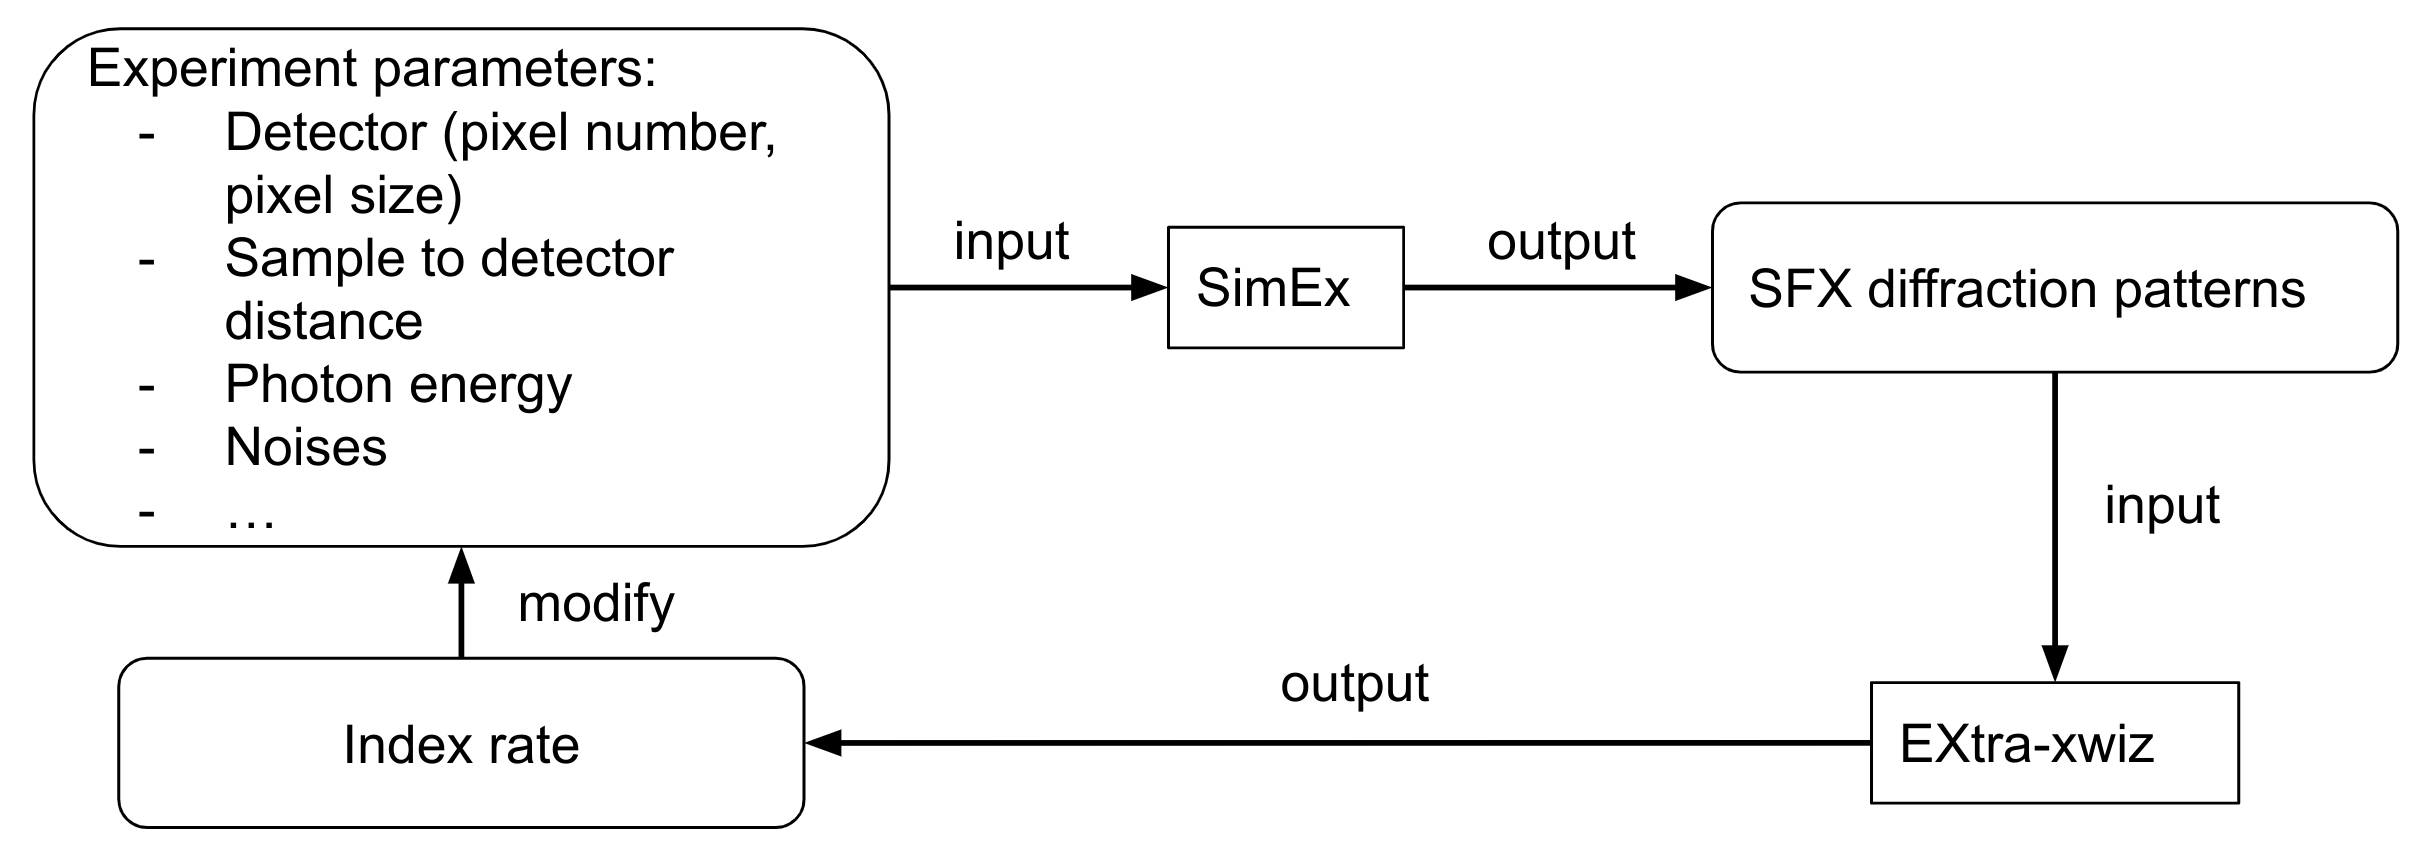
\includegraphics[width=0.75\columnwidth]{figures/feedbackloop.png}
    \caption{The schematic of the coupling of simulation software and data analysis tools.}
    \label{fig:feedbackloop}
\end{figure}
One of the workflow's use cases is to optimize the sample-to-detector distance for SFX experiments to reach the highest index rate within an acceptable range of resolution. We scanned several data points of sample-to-detector distance for the SFX simulation and analyzed the output with EXtra-xwiz to get the index rate in the corresponding condition (Fig.~\ref{fig:optSim}) With different X-ray energy densities, the sample-to-detector distance needed to reach the highest index rate is different. One can then optimize these parameters based on the exact need.
% {\color{blue}[The figure is currently just a place holder, the results will be updated next week.]} 

\begin{figure}[H]
\centering
\begin{flushleft}
\LARGE{(a)}
\end{flushleft}
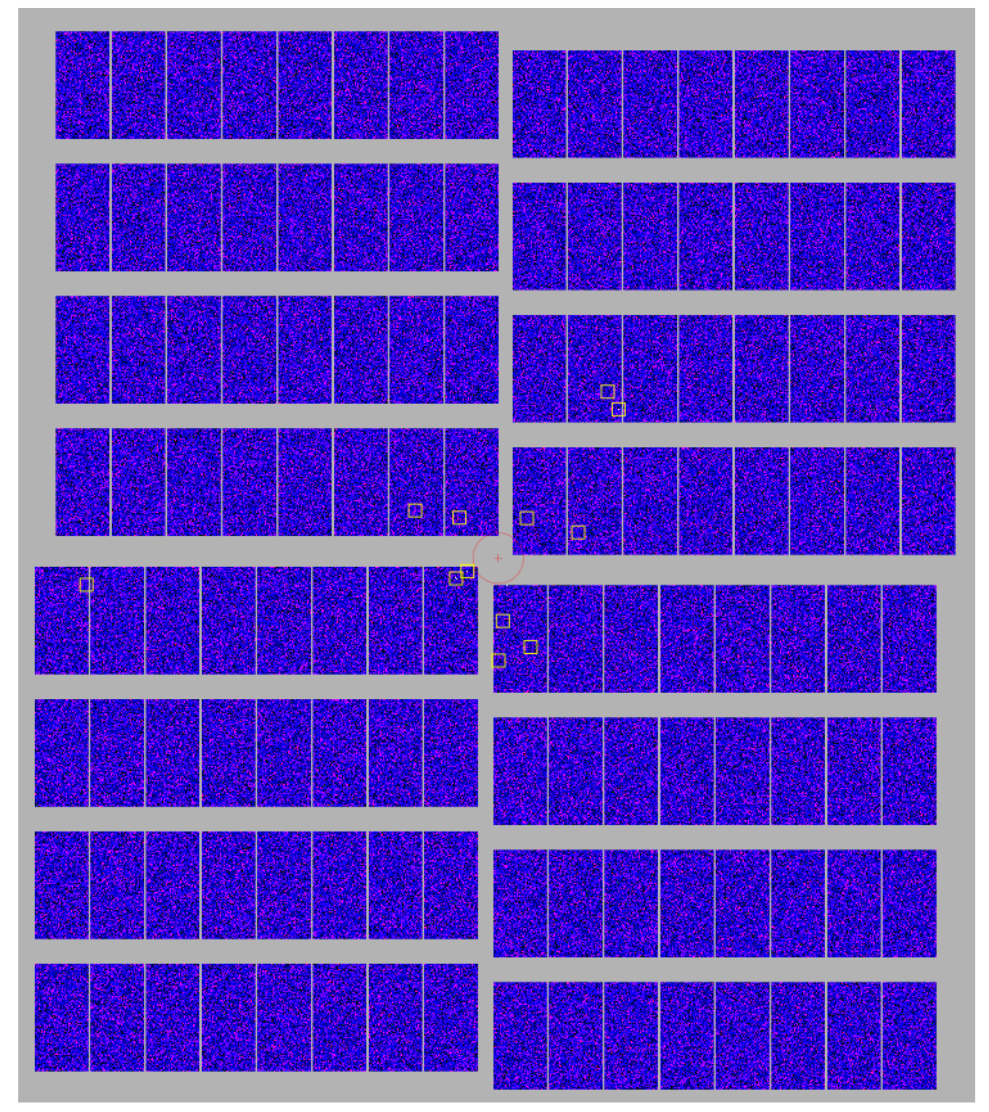
\includegraphics[width=0.6\textwidth]{figures/SFX_pattern.png} \\
\begin{flushleft}
\LARGE{(b)}
\end{flushleft}
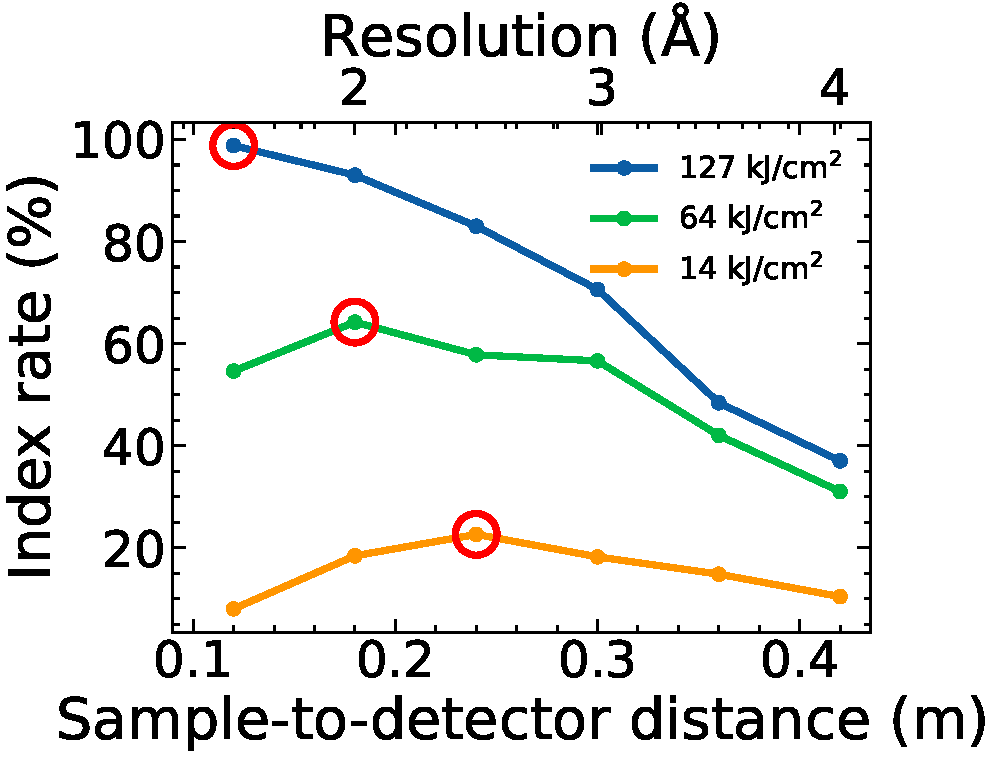
\includegraphics[width=0.6\textwidth]{figures/index_rate.pdf} 
\caption 
{\label{fig:optSim}
(a) An example SFX pattern for the simulation, the white rectangle boxes indicate found peaks. (b) The index rate curve as a function of the sample-to-detector distance with different X-ray energy densities.} 
\end{figure}


%%%%%%%%%%%%%%%%%%%%%%%%%%%%%%%%
% \bibliographystyle{unsrt}
% \bibliography{references}
\printbibliography


\end{document}
